\section*{Exercice 1 : L'utilisation des réseaux de Pétri pour le
  contrôle commande}
\subsection*{Question 1}
\textit{Cf.} figure $3$ de l'énoncé.
\subsection*{Question 2}
Notons $A_d$ et $R_d$ respectivement avancer et reculer le pochoir de
droite.  Notons $A_g$ et $R_g$ respectivement avancer et reculer le
pochoir de gauche.  Quand un pochoir avance, il ne recule pas.  On
commence donc pas le faire avancer ($p_3$ et $p_2$) puis reculer
($p_4$ et $p_5$) On distingue un bloc de parallélisme dans la figure 3
qui signifie que les pochoirs droite et gauche sont actionnés en
parallèle.

Au début d'un tour, en $p_1$, le pochoir ne reçoit aucun signal.  

Puis, en $t_1$, l'opération commence car on a les signaux $p$ et $q$ à
vrai. On rentre ensuite dans le bloc de parallélisme précédemment
décrit, jusqu'à $t_6$ où, après immobilisation à droite et à gauche
des pochoirs (places $p_6$ et $p_7$), un nouveau tour peut commencer
(retour en place $p_1$).
\subsection*{Question 3}
Le réseau de la figure $3$ est cohérent. En effet, de $p_1$ à $t_1$ un
seul jeton est en circulation. De $t_1$ à $t_6$ deux jetons sont en
circuation, mais dans une structure de type parallélisme (un jeton par
branche). En $t_6$, pour le retour à $p_1$, un seul jeton est à
nouveau en circulation. Chaque place ne reçoit donc qu'une seule
marque tout au long des évolutions du réseau.
\subsection*{Question 4}
Les combinaisons booléennes des signaux de sorties incompatibles sont
situées de manière séquentielle (et non parallèle). De plus, le réseau
est cohérent. Cela nous garantit ainsi l'exclusion mutuelle pour tous
les couples de places associés à ces étiquettes.
\subsection*{Question 5}
Le graphe des marquages accessibles associé au réseau de la figure $3$
est le suivant~:
$(p_1, p_2, p_3, p_4, p_5, p_6, p_7)$

\begin{center}
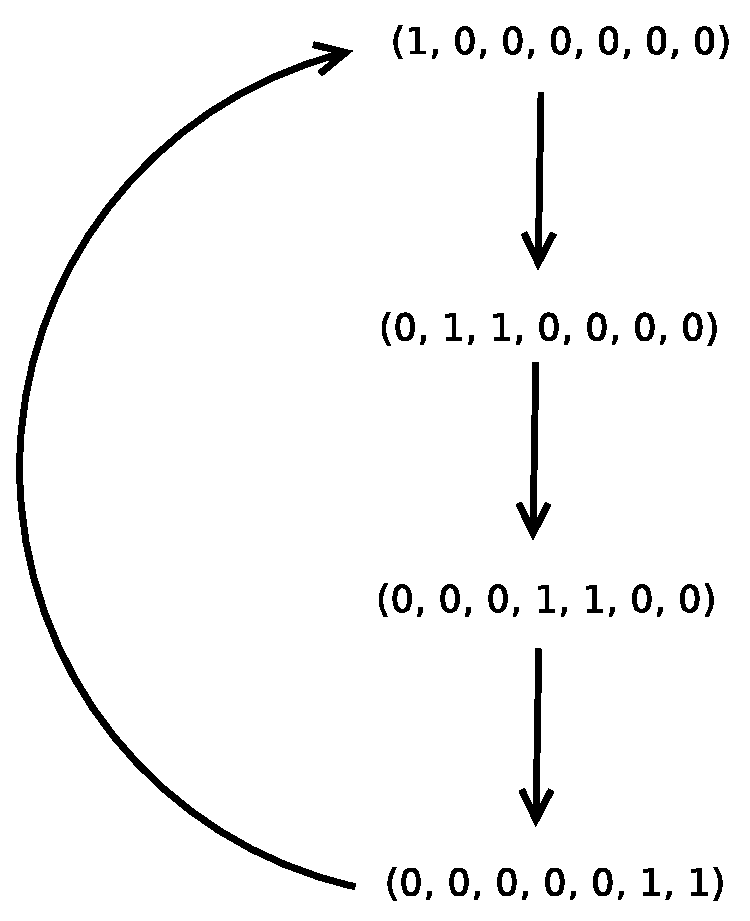
\includegraphics[height=6cm]{exo1_2.eps}
\end{center}

\subsection*{Question 6}
Matrice $C$ d'incidence du réseau de pétri de la figure $3$.

 $ \begin{pmatrix}
C&t_1&t_2&t_3&t_4&t_5&t_6 \\
p_1& -1&0&0&0&0&1 \\
p_2&1&-1&0&0&0&0 \\
p_3&1&0&-1&0&0&0 \\
p_4&0&1&0&-1&0&0 \\
p_5&0&0&1&0&-1&0 \\
p_6&0&0&0&0&1&-1 \\
p_7&0&0&0&1&0&-1 
\end{pmatrix}$

\subsection*{Question 7}
Calcul des P-semi flots associés au réseau de la figure
$3$. Appliquons pour cela l'algorithme de Farkas sur la matrice $C$
précédente.

On commence par  
$ \begin{pmatrix}
P& -1&0&0&0&0&1 \\
Q&1&-1&0&0&0&0 \\
R&1&0&-1&0&0&0 \\
S&0&1&0&-1&0&0 \\
T&0&0&1&0&-1&0 \\
U&0&0&0&0&1&-1 \\
V&0&0&0&1&0&-1 
\end{pmatrix}$

et l'on finit par trouver 
$ \begin{pmatrix}
P+Q+S& -1&0&1 \\
P+R+T&0&-1&0 \\
U&0&1&-1 \\
P+Q+S+V&0&0&0
\end{pmatrix}$
ce qui nous donne le P-semi flot $P+Q+S+V$, correspondant donc au
vecteur $(1, 1, 0, 1, 0, 0, 0, 1)$.

Par la suite, aucun autre P-semi flot ne peur être trouvé car, à
l'étape suivante, la matrice se réduit à
$ \begin{pmatrix}
P+R+T&-1&0 \\
U&1&-1
\end{pmatrix}$
\subsection*{Question 8}
Ce réseau n'admet pas de blocage car tout sommet est l'origine d'au
moins un arc.
\subsection*{Question 9}
Le réseau est bien un graphe d'évènement car chaque place possède une
seule transition d'entrée et une seule transition de sortie.

Les deux circuits élémentaires sont~:
\begin{itemize}
\item $p_1$ $\rightarrow$ $p_3$ $\rightarrow$ $p_5$ $\rightarrow$ $p_6$ $\rightarrow$ $p_1$
\item $p_1$ $\rightarrow$ $p_2$ $\rightarrow$ $p_4$ $\rightarrow$ $p_7$ $\rightarrow$ $p_1$
\end{itemize}
